\documentclass{llncs}

%\usepackage{polyglossia} % Must come before biblatex
\usepackage{algorithm}
\usepackage{algpseudocode}
\usepackage{amsfonts}
\usepackage{amsmath}
\usepackage{bm}
\usepackage{booktabs}
\usepackage{csquotes}
\usepackage[T1]{fontenc}
%\usepackage{fontspec}
\usepackage{graphicx}
\usepackage{hyperref}
%\usepackage{lua-visual-debug}
\usepackage{tabularx}


%\setdefaultlanguage{english}
%\setotherlanguage{czech}

\hypersetup{
	pdfencoding=auto,
	unicode=true,
	bookmarksopen=true,
	bookmarksopenlevel=3
}

\newcommand{\name}[1]{\textit{#1}}
\newcommand{\mathfield}{\ensuremath{\mathbb}}
\newcommand{\mathmat}{\ensuremath{\mathbf}}
\newcommand{\mathset}{\ensuremath{\mathbb}}
\newcommand{\mathspace}{\ensuremath{\mathcal}}
\newcommand{\mathvec}{\ensuremath{\bm}}

\newcounter{enumroman}
\newenvironment{romanitems}{\begin{list}{\bfseries(\roman{enumroman})\hfill}{\usecounter{enumroman}\setlength{\labelwidth}{\leftmargin}\addtolength{\labelwidth}{-1\labelsep}\topsep=0mm plus 2pt\itemsep=0mm\parsep=0mm plus 2pt\itemindent=0mm}}{\end{list}}

\DeclareMathOperator*{\argmin}{arg\,min}
\DeclareMathOperator*{\argmax}{arg\,max}


\usepackage{algorithm}
\usepackage{algpseudocode}

\begin{document}

\begin{algorithm*}
  \caption{The adaptive prolongation algorithm}
  \begin{algorithmic}
    \Require $ G_0 $ \Comment The original graph
    \Require $ \bm{y}_\mathrm{train} $ \Comment Training labels
    \Require $ n_p $ \Comment The number of nodes to prolong
    \Require $ \Psi_{i + 1} $ \Comment The previous embedding
    \Require $ \mathcal{C}_L^{(i + 1)}, \dots, \mathcal{C}_0^{(i + 1)} $ \Comment A list of all the contractions yet to be reversed
    \Ensure $ \Psi_i $ \Comment The next embedding
    \Ensure $ \mathcal{C}_L^{(i)}, \dots, \mathcal{C}_0^{(i)} $ \Comment Updated contraction list without the prolonged contractions
    \Statex
    \State $ node\_order \gets \Call{get\_node\_order}{G_0, \Psi_{i+1}, \bm{y}_\mathrm{train}, \mathcal{C}_L^{(i + 1)}, \dots, \mathcal{C}_0^{(i + 1)}} $
    \State $ \mathcal{C}_\mathrm{prolong} \gets \Call{select\_contractions}{node\_order, n_p, \mathcal{C}_L^{(i + 1)}, \dots, \mathcal{C}_0^{(i + 1)}} $
    \State $ \Psi_i \gets $ use $ \mathcal{C}_\mathrm{prolong} $ to prolong the embedding $ \Psi_{i + 1} $
    \State $ \mathcal{C}_L^{(i)}, \dots, \mathcal{C}_0^{(i)} \gets $ remove contractions in $ \mathcal{C}_\mathrm{prolong} $ from $ \mathcal{C}_L^{(i + 1)}, \dots, \mathcal{C}_0^{(i + 1)} $
    \Statex
    \Function{get\_node\_order}{$ G_0, \Psi_{i+1}, \bm{y}_\mathrm{train}, \mathcal{C}_L^{(i + 1)}, \dots, \mathcal{C}_0^{(i + 1)} $}
        \State $ \Psi_0^\mathrm{temp} \gets $ use $ \mathcal{C}_L^{(i + 1)}, \dots, \mathcal{C}_0^{(i + 1)} $ to fully prolong the current embedding $ \Psi_{i+1} $ to $ G_0 $
        \State $ model \gets \Call{train\_downstream\_model}{\Psi_0^\mathrm{temp}, \bm{y}_\mathrm{train}} $
        \State $ \mathmat{Y}_\mathrm{pred} \gets \Call{predict}{model, node} $ for each $ node \in V \left( G_0 \right) $
        \State $ entropy\_per\_node \gets H \left( \mathmat{Y}_\mathrm{pred} \right) $
        \State \Return $ V \left( G_0 \right) $, sorted in descending order by $ entropy\_per\_node $
    \EndFunction
    \Statex
    \Function{select\_contractions}{$ ordered\_nodes, n_p, \mathcal{C}_L^{(i + 1)}, \dots, \mathcal{C}_0^{(i + 1)} $}
        \State $ \mathcal{C}_\mathrm{prolong} \gets \left\{ \right\} $
        \For{$ node \in ordered\_nodes $, \textbf{until} $ \left\lvert \mathcal{C}_\mathrm{prolong} \right\rvert = n_p $}
            \State $ contraction \gets \Call{resolve\_contraction}{node, \mathcal{C}_\mathrm{prolong}, \mathcal{C}_L^{(i + 1)}, \dots, \mathcal{C}_0^{(i + 1)}} $
            \State If $ contraction \neq \mathrm{null} $, add $ contraction $ to $ \mathcal{C}_\mathrm{prolong} $
        \EndFor
        \State \Return $ \mathcal{C}_\mathrm{prolong} $
    \EndFunction
    \Statex
    \Function{resolve\_contraction}{$ node, \mathcal{C}_\mathrm{prolong}, \mathcal{C}_L^{(i + 1)}, \dots, \mathcal{C}_0^{(i + 1)} $}
        \State $ contraction \gets \mathrm{null} $
        \For{$ j \in \left\{ 0, \dots, L \right\} $} \Comment I.e. all steps of the original coarsening from finest to coarsest
            \State $ contraction\_candidate \gets $ find in $ \mathcal{C}_j^{(i + 1)} $ a contraction that affects $ node $, if not found, continue with $ j + 1 $
            \If{$ contraction\_candidate \in \mathcal{C}_\mathrm{prolong} $}
                \State \Return $ contraction $
            \EndIf
            \State $ contraction \gets contraction\_candidate $
            \State $ node \gets $ apply $ contraction $ to $ node $, so that in the next loop, a subsequent contraction may be selected
        \EndFor
        \State \Return $ contraction $
    \EndFunction
  \end{algorithmic}
\end{algorithm*}

\begin{figure*}
  \centering
  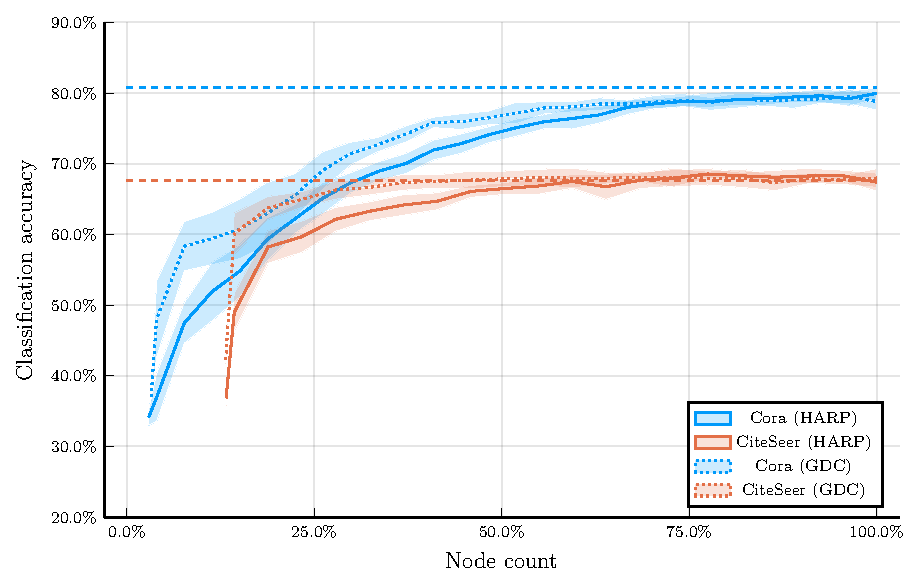
\includegraphics[width = \linewidth]{images/coarsening-algorithms/coarsening-algorithms.pdf}
  \caption{Downstream classifier accuracies at different steps of adaptive prolongation for different coarsening algorithms. Dashed line shows the baseline node2vec model accuracy. The node count is taken relative to the total node count in each dataset. The results are averaged over multiple runs, with the solid line representing the mean and the shaded area denoting one standard deviation.}
  \label{fig:adaptive-coarsening}
\end{figure*}

\end{document}
